\chapter{Nash Equilibrium Analysis}
\label{ch:nashanalysis}
This chapter presents a simulation that examines a system of agents competing to
sell electricity and its convergence to a Nash equilibrium.  Value function
based and policy gradient reinforcement learning algorithms are compared in
their convergence to an optimal policy using a six bus electric power system
model.

\section{Introduction}
This thesis presents the first case of
policy gradient reinforcement learning methods being applied to electricity
trading problems.  As a first step it is necessary to confirm that when using
these methods, a system of multiple agents will converge to the same Nash
equilibrium\footnote{Informally, a Nash equlibrium is a point in a
non-cooperative game at which no player is motivated to deviate from its
strategy, as it would result in lower gain \cite{nash50,nash51}.} that
a traditional closed-form simulation would produce.

This is the same approach used by \citeA{krause:nash06} before performing the
study of congestion management techniques that is reviewed in Section
\ref{sec:related_cong}.  Nash equilibria can be difficult
to determine in complex systems so the experiment presented here utilises a
model simple enough that it can be determined through exhaustive search.

By observing the actions taken and the reward received by each agent over the
initial simulation periods it is possible to compare the speed and consistency
with which different algorithms converge to an optimal policy. In the following
sections the objectives of the simulation are defined, the simulation setup
is explained and plots of results, with discussion and critical analysis, are
provided.

\section{Aims and Objectives}
Some elements of the simulations reported in this chapter are similar to those
presented by \citeA{krause:nash06}.  One initial aim of this work is to
reproduce their findings as a means of validating the approach.  The additional
objectives are to show:
\begin{itemize}
  \item That policy gradient methods converge to the same Nash equilibrium as
  value function based methods and tradtional closed-form simulations,
  \item Some the characteristics of policy gradient methods and how they differ
  from value function based methods.
%   \item The sensitivity of policy convergence to algorithm parameter choices
%   and policy function approximation structure.
\end{itemize}
Meeting these objectives aims to provide a basis for using policy gradient
methods in more complex simulations, to show that they can learn basic policies
and to provide guidance for algorithm parameter selection.

\section{Method of Simulation}
% Each learning method is tested individually using a range of parameter
% configurations.  A power system model with one bus, one generator $k$ and
% one dispatchable load $l$.  In this
% context, the market clearing process is equivalent to creating offer and bids
% stacks and finding the point of intersection.  A passive agent is associated
% with the dispatchable load.  This agent bids for $-p_{g,l}^{min}$ at marginal
% cost each period regardless of environment state or reward signal.  A
% dispathcable load is used instead of a constant load to allow a price to be
% set. Generator $k$ is given sufficient capacity to supply the demand
% of the dispatchable load, $p_{g,k}^{max} > -p_{g,l}^{min}$, and the marginal of
% the $k$ is half that of the load $l$.  The generator and dispatchable load
% attributes are given in Table X.  A price cap for the market is set to twice the
% marginal cost of the $l$ at full capacity, $p_{g,l}^{min}$.  The DC optimal
% power flow formulation (See Section \ref{sec:opf}, above) is used to clear the
% market and reactive power trade is omitted.
Learning methods are compared in this chapter by repeating the same
simulation with different algorithms used by the agents.  An alternative
might be to use a combination of methods in the same simulation, but the
approach used here is intended to be an extension of the work by
\citeA{krause:nash06}.

Each simulation uses a six bus electric power system model adapted from
\citeA[pp.~104, 112, 119, 123-124, 549]{wood:pgoc}.  The model provides a simple
environment for electricity trade with a small number of generators and branch
flow constraints that slightly increase the complexity of the Nash equilibria.
The buses are connected by eleven transmission lines at 230kV. The model
contains three generating units with a total capacity of 440MW and loads at
three locations, each 70MW in size. The connectivity of the branches and the
locations of the generators and loads is shown in Figure~\ref{fig:case6ww}. Data
for the power system model was taken from a case provided with \textsc{Matpower}
and is listed in Appendix \ref{adx:case6ww}.

Two sets of quadratic generator operating cost functions, of the form
$c(p_i)=ap_i^2+bp_i+c$ where $p_i$ is the output of generator $i$, are defined
in order to create two different equilibria for investigation.  The coefficients
$a$, $b$ and $c$ for cost configuration 1 are listed in Table
\ref{tbl:case6ww_gencost1}.  This configuration defines two low cost
generators that can not offer a price greater than the marginal cost of the most
expensive generator when they apply the maximum possible markup. The set of
coefficients for cost configuration 2 is listed in Table
\ref{tbl:case6ww_gencost2}.  This configuration narrows the cost differences
such that offer prices may overlap and may exceed the marginal cost of the most
expensive generator.
% To strengthen the penalty for not being dispatched and
% shutdown cost $C_{down}$ of \$100 is specified in this configuration.

\ifthenelse{\boolean{includefigures}}{\begin{figure}
\label{fig:case6ww}
\centering
\begin{scriptsize}
\begin{tikzpicture}[thick]

\coordinate (c1) at (0,4);
\coordinate (c2) at (5,6.5);
\coordinate (c3) at (10,4);
\coordinate (c4) at (0,0);
\coordinate (c5) at (5,-2.5);
\coordinate (c6) at (10,0);
\coordinate (over) at (0,3.75);

\busbar{b1}{c1}{20mm}
\busbar{b2}{c2}{30mm}
\busbar{b3}{c3}{20mm}
\busbar{b4}{c4}{20mm}
\busbar{b5}{c5}{30mm}
\busbar{b6}{c6}{20mm}

% Branch 1-2.
\draw[line] ([xshift=5mm] b1.north) node[rotate=90,above right]{$15.41$}
node[rotate=90,below right]{$-9.58$} -- ++(0,3.75) -| ([xshift=-8mm] b2.north)
node[rotate=90,above right]{$-15.14$} node[rotate=90,below right]{$5.70$};
% Branch 1-4.
\draw[line] ([xshift=-5mm] b1.south) node[rotate=90,above left]{$33.95$}
node[rotate=90,below left]{$22.50$} -- ([xshift=-5mm] b4.north)
node[rotate=90,above right]{$-33.15$} node[rotate=90,below right]{$-23.46$};
% Branch 1-5.
\draw[line] ([xshift=5mm] b1.south) node[rotate=90,above left]{$27.86$}
node[rotate=90,below left]{$12.80$} -- ([xshift=5mm,yshift=-15mm] b1.south)
-- ([xshift=-8mm,yshift=15mm] b5.north) -- ([xshift=-8mm] b5.north)
node[rotate=90,above right]{$-27.11$} node[rotate=90,below right]{$-16.20$};
% Branch 2-3.
\draw[line] ([xshift=8mm] b2.north) node[rotate=90,above right]{$0.29$}
node[rotate=90,below right]{$-11.76$} -- ++(0,1.25) -| ([xshift=-5mm] b3.north)
node[rotate=90,above right]{$-0.25$} node[rotate=90,below right]{$5.18$};
% Branch 2-4.
\draw[line,ultra thick] ([xshift=-8mm] b2.south) node[rotate=90,above
left]{$41.74$} node[rotate=90,below left]{$43.11$} --
([xshift=-8mm,yshift=-15mm] b2.south) -- node[sloped,above]{$\vert S_{max}^5
\vert = 60.0$} ([xshift=5mm,yshift=15mm] b4.north) -- ([xshift=5mm] b4.north)
node[rotate=90,above right]{$-40.06$} node[rotate=90,below right]{$-41.83$};
% Branch 2-5.
\draw[line] (b2.south) node[rotate=90,above left]{$17.35$}
node[rotate=90,below left]{$14.93$} -- (b5.north) node[rotate=90,above
right]{$-16.81$} node[rotate=90,below right]{$-17.46$};
% Branch 2-6.
\draw[line] ([xshift=8mm] b2.south) node[rotate=90,above left]{$25.03$}
node[rotate=90,below left]{$12.67$} -- ([xshift=8mm,yshift=-15mm] b2.south)
-- ([xshift=-5mm,yshift=15mm] b6.north) -- ([xshift=-5mm] b6.north)
node[rotate=90,above right]{$-24.49$} node[rotate=90,below right]{$-16.38$};
% Branch 3-5.
\draw[line] ([xshift=-5mm] b3.south) node[rotate=90,above left]{$23.18$}
node[rotate=90,below left]{$21.57$} -- ([xshift=-5mm,yshift=-15mm] b3.south)
-- ([xshift=8mm,yshift=15mm] b5.north) -- ([xshift=8mm] b5.north)
node[rotate=90,above right]{$-21.99$} node[rotate=90,below right]{$-24.28$};
% Branch 3-6.
\draw[line] ([xshift=5mm] b3.south) node[rotate=90,above left]{$47.50$}
node[rotate=90,below left]{$59.90$} -- ([xshift=5mm] b6.north)
node[rotate=90,above right]{$-46.45$} node[rotate=90,below right]{$-56.82$};
% Branch 4-5.
\draw[line] ([xshift=5mm] b4.south) node[rotate=90,above left]{$3.21$}
node[rotate=90,below left]{$-4.71$} -- ++(0,-3.75) -| ([xshift=-8mm] b5.south)
node[rotate=90,above left]{$-3.19$} node[rotate=90,below left]{$-3.03$};
% Branch 5-6.
\draw[line] ([xshift=8mm] b5.south) node[rotate=90,above left]{$-0.90$}
node[rotate=90,below left]{$-9.03$} -- ++(0,-1.25) -| ([xshift=-5mm] b6.south)
node[rotate=90,above left]{$0.94$} node[rotate=90,below left]{$3.21$};

% Generator 1.
\genset{g1}{$(c1)+(-5mm,15mm)$}
\draw[line] ([xshift=-5mm] b1.north) -- node[sloped,above]{$77.22$}
node[sloped,below]{$25.72$} (g1.south);
% Generator 2.
\genset{g2}{$(c2)+(0,15mm)$}
\draw[line] (b2.north) -- node[sloped,above]{$69.27$}
node[sloped,below]{$64.65$} (g2.south);
% Generator 3.
\genset{g3}{$(c3)+(5mm,15mm)$}
\draw[line] ([xshift=5mm] b3.north) -- node[sloped,above]{$70.42$}
node[sloped,below]{$86.64$} (g3.south);

% Load 1.
\loadd{l1}{$(c4)-(5mm,15mm)$}
\draw[line] (l1.south) -- node[sloped,above]{$70.00$}
node[sloped,below]{$70.00$} ([xshift=-5mm] b4.south);
% Load 2.
\loadd{l2}{$(c5)-(0mm,15mm)$}
\draw[line] (l2.south) -- node[sloped,above]{$70.00$}
node[sloped,below]{$70.00$} (b5.south);
% Load 3.
\loadd{l3}{$(c6)+(5mm,-15mm)$}
\draw[line] (l3.south) -- node[sloped,above]{$70.00$}
node[sloped,below]{$70.00$} ([xshift=5mm] b6.south);

\end{tikzpicture}
\end{scriptsize}
\caption{One line diagram for six bus power system model from [].}
\end{figure}
}{}

\begin{table}
\begin{center}
\begin{tabular}{c|c|c|c|c}
\hline
Gen &$C_{down}$ &$a$ &$b$ &$c$ \\
\hline\hline
 1 &0 &0.0 &4.0 &200.0 \\
 2 &0 &0.0 &3.0 &200.0 \\
 3 &0 &0.0 &6.0 &200.0 \\
\hline
\end{tabular}
\caption{Generator cost configuration 1.}
\label{tbl:case6ww_gencost1}
\end{center}
\end{table}

\begin{table}
\begin{center}
\begin{tabular}{c|c|c|c|c}
\hline
Gen &$C_{down}$ &$a$ &$b$ &$c$ \\
\hline\hline
 1 &0 &0.0 &5.1 &200.0 \\
 2 &0 &0.0 &4.5 &200.0 \\
 3 &0 &0.0 &6.0 &200.0 \\
\hline
\end{tabular}
\caption{Generator cost configuration 2.}
\label{tbl:case6ww_gencost2}
\end{center}
\end{table}

As in \citeA{krause:nash06}, no load profile is defined for the simulation. The
system load is assumed to be peak in all periods and only one state is defined
for methods using look-up tables.  Each simulation step is assumed to be one
hour in length.

For all generators $P^{min}=0$ so as to simplify the equilbria and avoid the
need to use the unit de-commitment algorithm.  The maximum capacity for the most
expensive generator $P^{max}_3=220$MW such that it may almost supply all of the
load if dispatched.  This generator is associated with a passive agent that
always offers full capacity at marginal cost.  For the less expensive generators
$P^{max}_1=P^{max}_2=110$MW.  These two generators are each associated with an
active learning agent whose activity in the market is restricted to one offer of
maximum capacity in each period, at a price representing a markup of between 0
and 30\% on marginal cost.  Methods restricted to discrete actions may markup in
steps of 10\%, giving possible markup actions of 0, 10\%, 20\% and 30\%.  No
capacity withholding is implemented.
% The market price cap is set such that it is never reached by any markup and
% does not complicate the experiment.
Discriminatory pricing (pay-as-bid) is used in order to provide a clearer reward
signal to agents with low cost generators.

The algorithms which are compared are Q-learning, ENAC, REINFORCE and the
modified Roth-Erev technique (See Section \ref{sec:rl}). Default algorithm
parameter values from PyBrain are used and no attempt to study parameter sensitivity or variations in function approximator
design is made.

For the Q-learning algorithm $\alpha=0.3$, $\gamma=0.99$ and $\epsilon$-greedy
action selection is used with $\epsilon=0.9$ and $d=0.98$.  For the Roth-Erev
technique $\epsilon=0.55$, $\phi=0.3$ and Boltzmann action selection is used
with $\tau=100$ and $d=0.99$.

Both REINFORCE and ENAC use a two-layer neural network with one linear input
node, one linear output node, no bias nodes and with the connection weight
initialised to zero.  A two-step episode is defined for the policy gradient
methods and five episodes are performed per learning step.  The exploration
parameter $\sigma$ for these methods is initialised to zero and adjusted
manually after each episode such that:
\begin{equation}
\label{eq:sigmadecay}
\sigma_{t} = d(\sigma_{t-1}-\sigma_{n})+\sigma_{n}
\end{equation}
where $d=0.998$ is a decay parameter and $\sigma_{n}=-0.5$ specifies the
value that is converged to asymtotically.  In each simulation the learning rate
$\gamma=0.01$ for the policy gradient methods, apart from for ENAC under cost
configuration 2 where $\gamma=0.005$.  Both active agents use the same
parameter values in each simulation.

As in \citeA{krause:nash06}, the point of Nash equilibrium is established by
computing each agent's reward for all possible combinations of discrete markup.
The rewards for Agent 1 and Agent 2 under cost configuration 1 are given in Table
\ref{tbl:nash1}.  The Nash equilibrium points are marked with a *.  The table
shows that the optimal policy for each agent is to apply the maximum markup to
each offer as their generators are always dispatched.
The rewards under cost configuration~2 are given in Table \ref{tbl:nash2}. This
table shows that the optimal point occurs when Agent 2 applies its maximum
markup and Agent 1 offers a price just below the marginal cost of the passive agent's
generator.

\begin{table}
\begin{center}
\begin{small}
\begin{tabular}{c.{2.2}|.{2.1}.{2.1}|.{2.1}.{2.1}|.{2.1}.{2.1}|.{3.1}.{2.1}|}
\cline{3-10}
 & &\multicolumn{8}{c|}{$G_1$} \\
\cline{3-10}
 & &\multicolumn{2}{c|}{0.0\%} &\multicolumn{2}{c|}{10.0\%} &\multicolumn{2}{c|}{20.0\%} &\multicolumn{2}{c|}{30.0\%} \\
 & &r_1 &r_2 &r_1 &r_2 &r_1 &r_2 &r_1 &r_2 \\
\hline
\multicolumn{1}{|c|}{\multirow{4}{*}{$G_2$}} &0.0\% &0.0 &0.0 &40.0 &0.0 &80.0 &0.0 &120.0 &0.0 \\
\multicolumn{1}{|c|}{} &10.0\% &0.0 &33.0 &40.0 &33.0 &80.0 &33.0 &120.0 &33.0 \\
\multicolumn{1}{|c|}{} &20.0\% &0.0 &66.0 &40.0 &66.0 &80.0 &66.0 &120.0 &66.0 \\
\multicolumn{1}{|c|}{} &30.0\% &0.0 &99.0 &40.0 &99.0 &80.0 &99.0 &120.0^*
&99.0^* \\
\hline
\end{tabular}
\caption{Agent rewards under cost configuration~1}
\label{tbl:nash1}
\end{small}
\end{center}
\end{table}

\begin{table}
\begin{center}
\begin{small}
\begin{tabular}{c.{2.2}|.{2.1}.{3.1}|.{2.1}.{3.1}|.{2.1}.{3.1}|.{2.1}.{3.1}|}
\cline{3-10}
 & &\multicolumn{8}{c|}{$G_1$} \\
\cline{3-10}
 & &\multicolumn{2}{c|}{0.0\%} &\multicolumn{2}{c|}{10.0\%} &\multicolumn{2}{c|}{20.0\%} &\multicolumn{2}{c|}{30.0\%} \\
 & &r_1 &r_2 &r_1 &r_2 &r_1 &r_2 &r_1 &r_2 \\
\hline
\multicolumn{1}{|c|}{\multirow{4}{*}{$G_2$}} &0.0\% &0.0 &0.0 &51.0 &0.0 &0.0 &0.0 &0.0 &0.0 \\
\multicolumn{1}{|c|}{} &10.0\% &0.0 &49.5 &51.0 &49.5 &0.0 &49.5 &0.0 &49.5 \\
\multicolumn{1}{|c|}{} &20.0\% &0.0 &92.2 &51.0 &99.0 &0.0 &99.0 &0.0 &99.0 \\
\multicolumn{1}{|c|}{} &30.0\% &0.0 &126.8 &54.8^* &138.4^* &0.0 &148.5 &0.0
&148.5 \\
\hline
\end{tabular}
\caption{Agent rewards under cost configuration~2}
\label{tbl:nash2}
\end{small}
\end{center}
\end{table}

\section{Simulation Results}
Each action taken by an agent and the consequent reward is recorded for each
simulation.  Values are averaged over the ten simulation runs and standard
deviations are calculated using the formula
\begin{equation}
SD = \sqrt{\frac{1}{N-1}\sum_{i=0}^{N}(x_i - \bar{x})^2}
\end{equation}
where $x_i$ is the action or reward value in simulation $i$ of $N$ simulation
runs and $\bar{x}$ is the mean of the values.

Figure \ref{fig:5_1_action_a1} shows the average markup on marginal cost and the
standard deviation over the ten simulation runs for Agent 1 under price
configuration 1, using the four learning methods.  The second $y$-axis in each
plot relates to the exploration parameter for each method.  Figure
\ref{fig:5_1_action_a2} shows the same information for Agent 2.  Plots of
reward are not given as generator prices and the market are configured such that an
agent's reward is directly proportional to its action.  The plots are vertically
aligned and have equal $x$-axis limits to assist algorithm comparison.

\ifthenelse{\boolean{includefigures}}{
	\begin{figure}
	  \centering
	  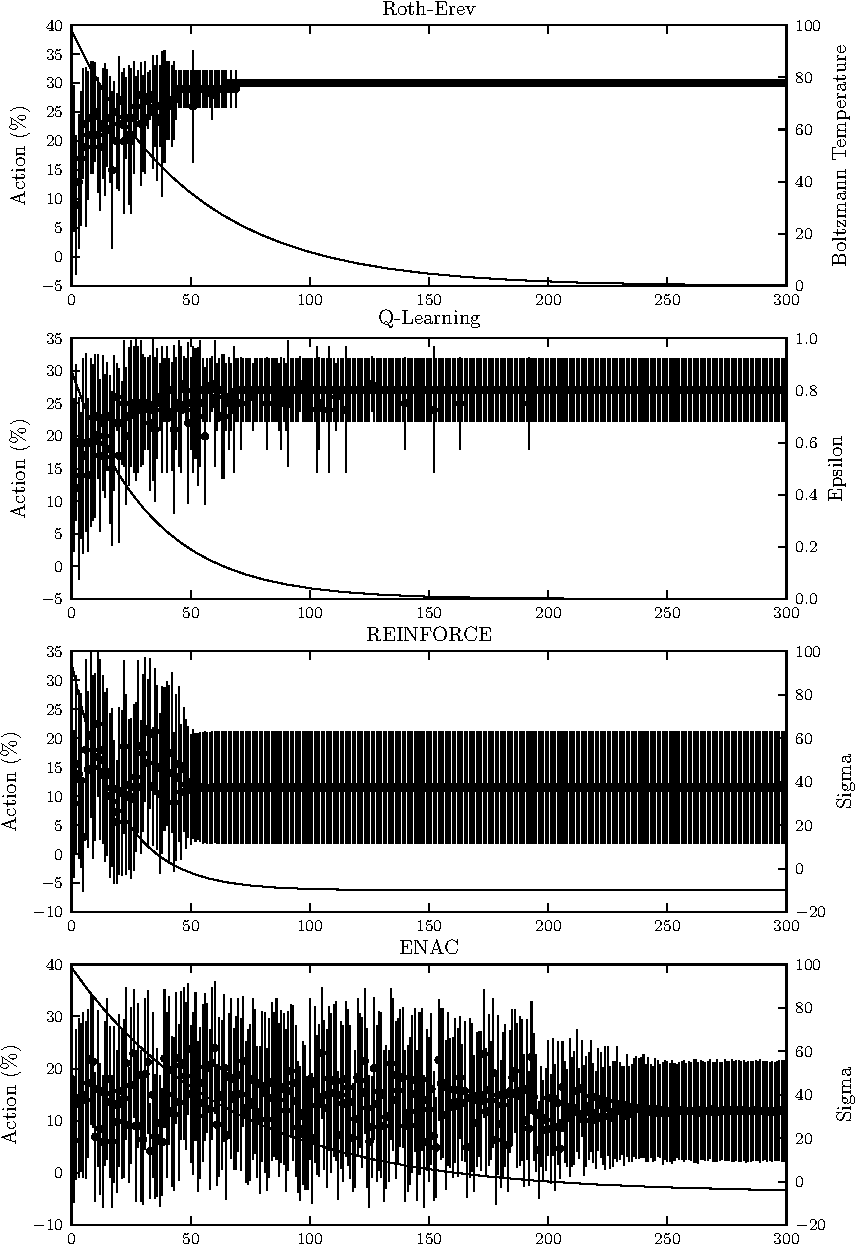
\includegraphics{figures/fig5_1_action_a1}
	  \caption{Average markup for agent 1 and standard deviation over 10 runs.}
	  \label{fig:5_1_action_a1}
	\end{figure}

	\begin{figure}
	  \centering
	  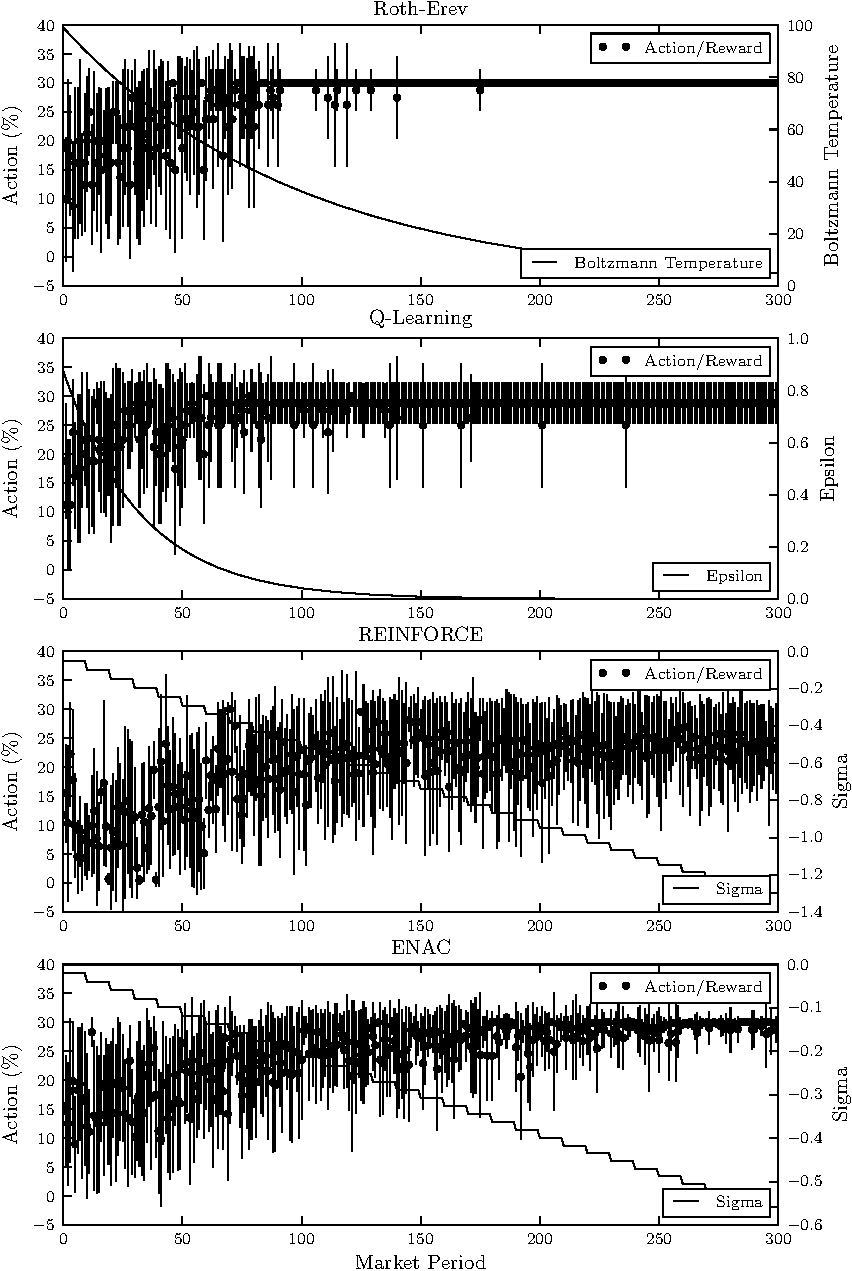
\includegraphics{figures/fig5_1_action_a2}
	  \caption{Average markup for agent 2 and standard deviation over 10 runs.}
	  \label{fig:5_1_action_a2}
	\end{figure}
}{}

Figures \ref{fig:5_2_action_a1} and \ref{fig:5_2_reward_a1} plot the average
markup and reward over ten simulation runs for Agent 1 and Agent 2,
respectively, under price configuration 2 for the variant Roth-Erev,
Q-learning learning methods.  The plots for REINFORCE and ENAC in these figures
are for actual values in one simulation run as the number of interactions and
variation in values makes the results difficult to observe otherwise.
%Not all $x$-axis extents are equal in these two figures.

\ifthenelse{\boolean{includefigures}}{
	\begin{figure}
	  \centering
	  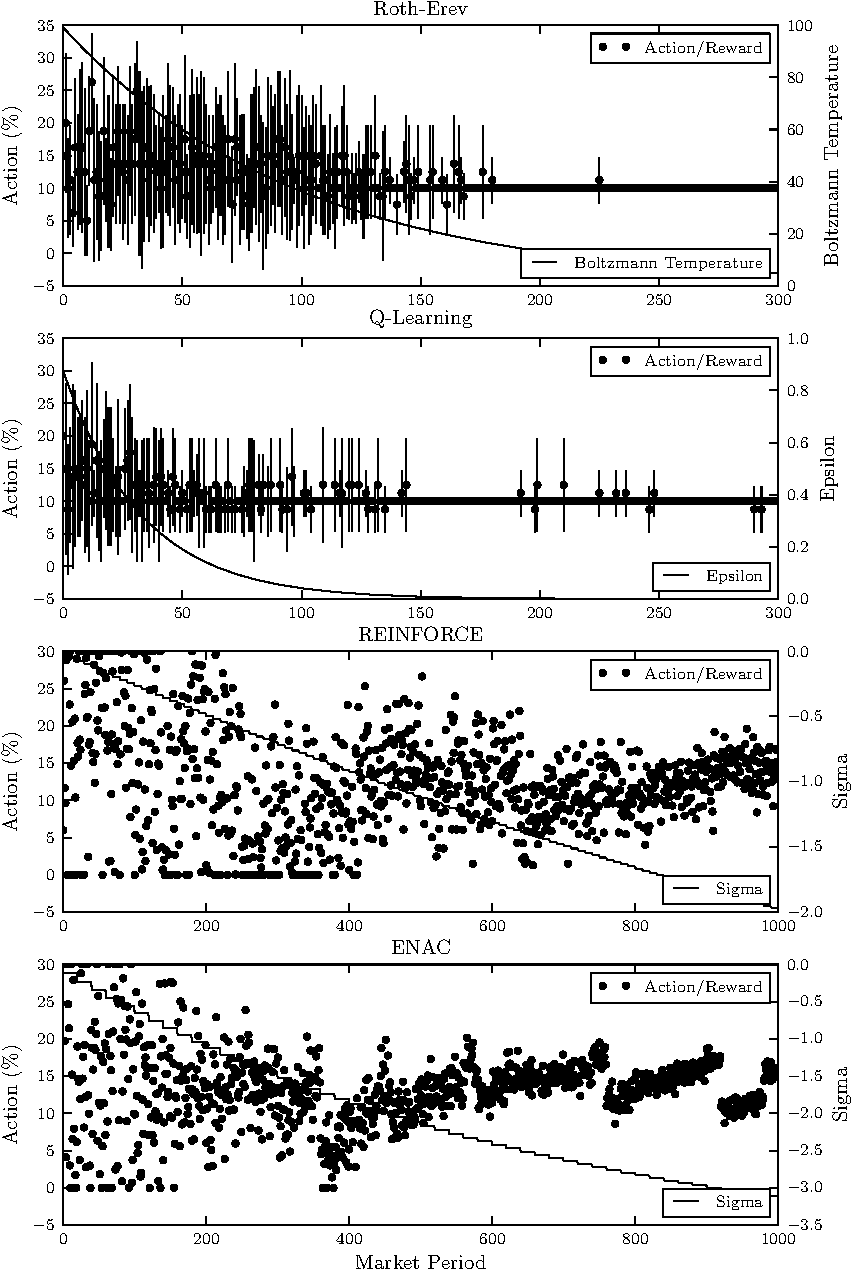
\includegraphics{figures/fig5_2_action_a1}
	  \caption{Average markup for agent 1 and standard deviation.}
	  \label{fig:5_2_action_a1}
	\end{figure}
% 	\begin{figure}
% 	  \centering
% 	  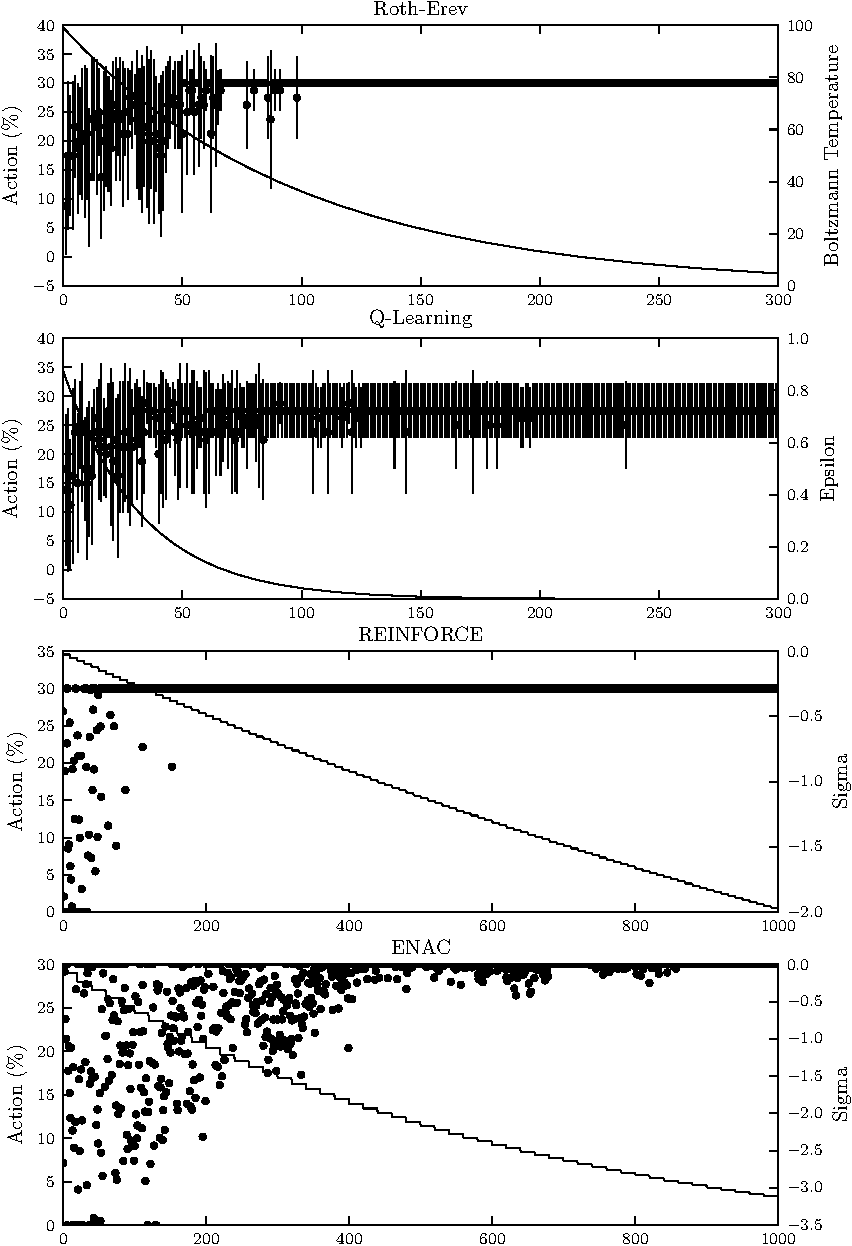
\includegraphics{figures/fig5_2_action_a2}
% 	  \caption{Average markup for agent 2 and standard deviation.}
% 	  \label{fig:5_2_action_a2}
% 	\end{figure}
	\begin{figure}
	  \centering
	  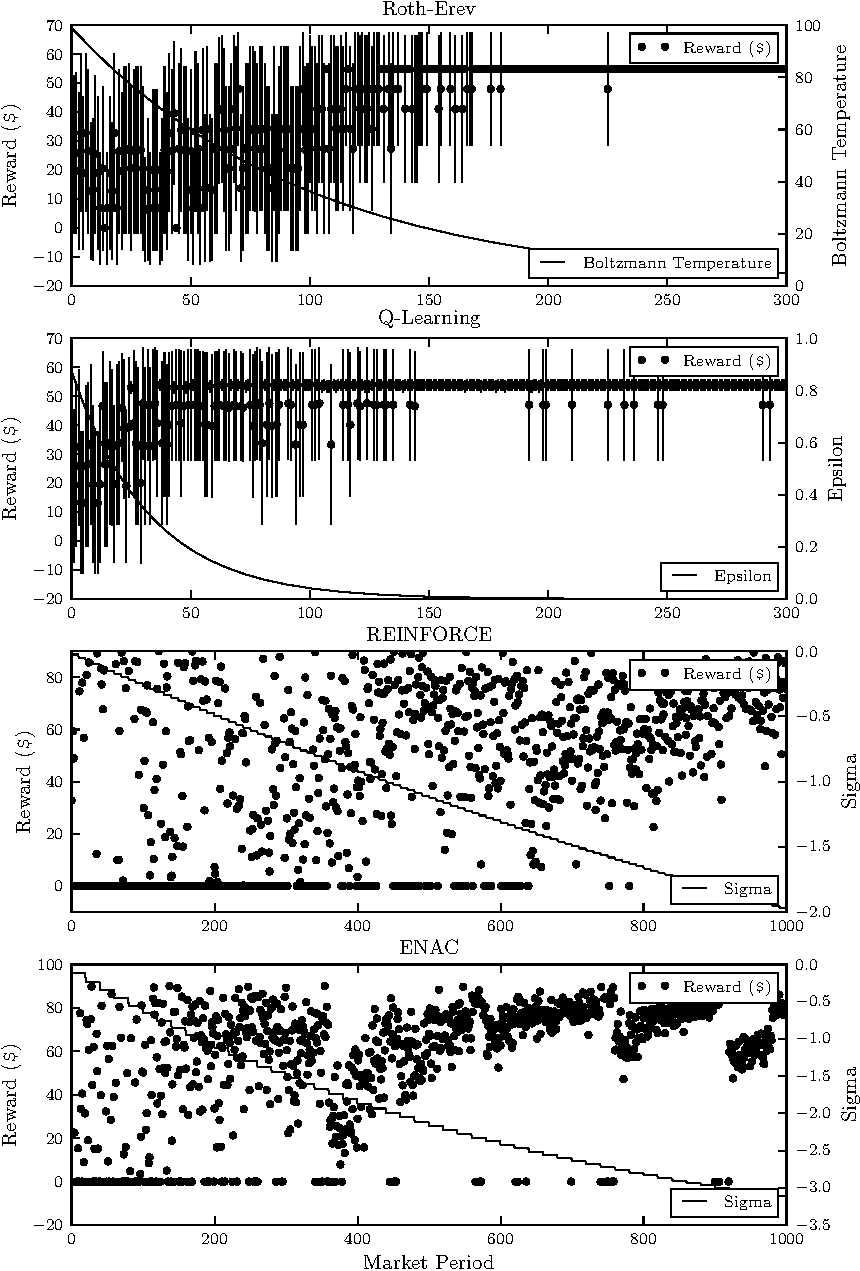
\includegraphics{figures/fig5_2_reward_a1}
	  \caption{Average reward for agent 1 and standard deviation.}
	  \label{fig:5_2_reward_a1}
	\end{figure}
% 	\begin{figure}
% 	  \centering
% 	  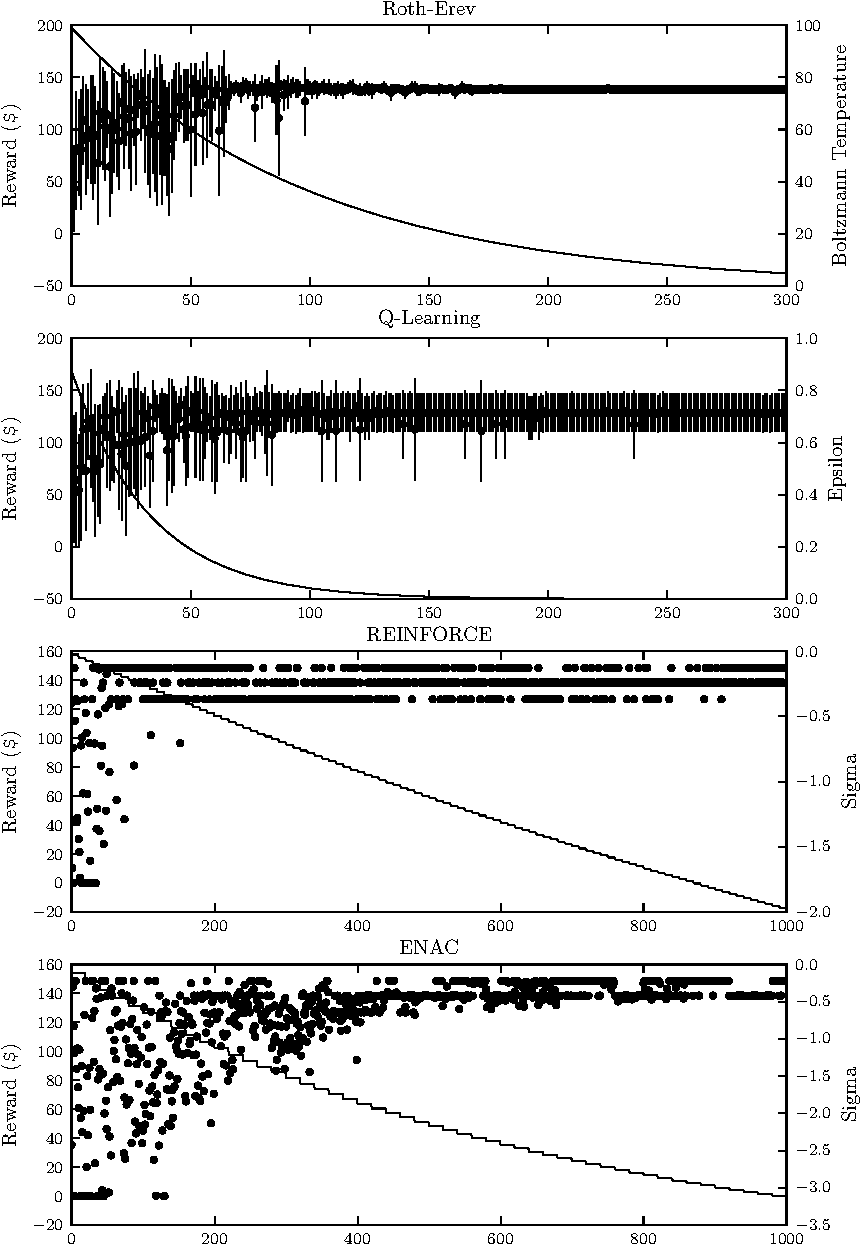
\includegraphics{figures/fig5_2_reward_a2}
% 	  \caption{Average reward for agent 2 and standard deviation.}
% 	  \label{fig:5_2_reward_a2}
% 	\end{figure}
}{}

\section{Discussion and Critical Analysis}
Under cost configuration 1 the agents face a relatively simple control task and
receive a clear reward signal that is directly proportional to their markup. The
results show that all of the methods consistently converge to the point of Nash
equilibrium.  The variant Roth-Erev method shows very little variation
around the mean once converged, due to the use of Boltzmann exploration with a
then low temperature parameter value.  The constant variation around the mean
that can be seen for Q-learning once converged is due to the use of
$\epsilon$-greedy action selection and can be removed if a Boltzmann explorer
is used.

Empirical studies have also shown that the speed of convergence is largely
determined by the rate at which the exploration parameter value is reduced.
However, the episodic nature of the policy gradient methods requires them to
make several interactions per learning step and therefore a larger number of
initial exploration steps are needed.  Policy gradient methods have also been
found to be highly sensitive to the choice of learning rate.  High
values cause large changes to policy parameters to be made at each step and
may cause the algorithm to not converge, but low values cause the
algorithm to learn very slowly.

Cost configuration 2 provides a more challenging control problem in which
Agent~1 must learn to undercut the passive agent.  The results show that the
variant Roth-Erev and Q-learning methods both consistently learn their optimal
policy and converge to the Nash equilibrium.  However, there is space for
Agent~1 to markup its offer by slightly more than 10\% and still undercut the
passive agent, but methods with discrete actions are not able to exploit this
and do not receive the additional profit.

The results for the policy gradient methods under cost configuration 2 show that
they learn to reduce their markup if their offer price starts to exceed
that of the passive agent and the reward signal drops.  However, a chattering
effect below the Nash equilibrium point can be clearly seen for ENAC and the
method does not learn to always undercut the other agent.  These methods also
require a much larger number of simulation steps and for the exploration
parameter to decay slowly if they are to produce this behaviour.  This
is due to the need for a lower learning rate that ensures fine policy
adjustments can be made and for several interactions to be performed between
each learning step.
% When using REINFORCE or ENAC, Agent~2 tends also to learn to maximise its
% markup, but less consistently.  Agent~1 typically learns to undercut the
% passive agent, but does not converge to a consistent value.  The problem is
% similar to the cliff-edge walking problems often used as benchmarks in
% reinforcement learning research and may be difficult to approximate a policy
% for using a small number of $\tanh$ functions. It may be possible to improve
% the performance of these agents through more educated policy function
% approximator design. but these methods are not really intended for operation
% in such simple environments.

\section{Summary}
By observing the state to which a multi-learning-agent system converges, it is
possible to verify that learning algorithms produce the same Nash equilibrium
that closed-form simulations provide.  The results presented in this chapter closely
correspond with those from \citeA{krause:nash06} for Q-learning and show
equivalent behaviour for the variant Roth-Erev method.  The simulations
illustrate how challenging unsupervised learning in a continuous environment can
be, even for simple problems. Tasks in which a large reward change can occur for
a very small change in policy prove difficult for policy gradient methods to
learn and require low learning rates and lengthy periods of exploration.  The
operation of policy gradient methods with noisy, multi-dimensional state data
is not examined in this chapter and deserves investigation.

% This experiment confirms the convergence to a Nash equilibrium of the
% Q-learning methods that is published in \citeA{krause:nash06} and, to a degree,
% extends the conclusion to policy gradient methods.  The results show that
% while these methods do converge to the same or similar policies as the
% Q-learning and Roth-Erev methods, they do not exhibit the same level of
% consistency.  Value function based methods or the Roth-Erev method may be the
% most suitable choice of algorithm in the simple electricity market simulations
% typically found in the literature.
%
% The simulations conducted here do not exploit any of the abilities of policy
% gradient methods to utilise multi-dimensional continuous state information and
% their behaviour in more complex electricity market environments deserves
% investigation.

%\section{Summary}


% \chapter{Competitive Power Trade}
% Having compared the learning methods in a one-player context, this section
% describes the method used to pit them against one and other and compare their
% performance.
%
% \section{Aims \& Objectives}
% Competition is fundamental to markets and this experiment aims to compare
% learning methods in a complex dynamic market environment with multiple
% competing participants.  The objective is to compare:
% \begin{itemize}
%   \item Performance, in terms of profitability, over a finite number of
%   periods,
%   \item Profitability when trading both active and reactive power.
%   \item Consistency of profit making and,
%   \item Sensitivity to algorithm parameter changes.
% \end{itemize}
%
% \section{Method of Simulation}
% Figure X illustrates the structure of the six bus power system model, from
% \cite{wood:pgoc}, with three generators and fixed demand at three of the buses
% used to provide a dynamic environment with typical system values.  Bus,
% branch and generator attribute values are stated in Tables X, Y, Z,
% respectively.  Three learning methods are compared in six simulations
% encapsulating all method--generator combinations.
%
% A price cap $c_{cap}$ of twice the marginal cost of the most expensive generator
% at full capacity is set by the market.  The simulations are repeated for with agents
% actions composing both price and quantity and with just price.  For the
% value-function methods, the state is defined by the market clearing price from
% the previous period, divided equally into $x_s$ discrete states between $0$ and
% $c_{cap}$.  The state vector $s_t$ for the policy gradient methods consists of
% the market clearing price and generator set-point from the previous period.
% \begin{equation}
% s_t =
% \begin{bmatrix}
% c_{mcp}\\
% p_g
% \end{bmatrix}
% \end{equation}
% The script used to conduct the simulation is provided in Listing X.

\chapter{System Constraint Exploitation}
\label{ch:exploitation}
% One of the main features of agents using policy gradient learning methods and
% artifical neural networks for policy function approximation is their ability
% to accept many signals of continuous sensor data.  This section describes an
% experiment in which the power system is severly constrained for certain
% periods, resulting in elevated nodal marginal prices in particular areas.  The
% methods are tested in their ability to exploit these constraints and improve
% their total accumulated reward.
This chapter explores the exploitation of constraints by learning agents in a
dynamic electricity trading environment.  Value function based and policy
gradient reinforcement learning methods are compared using a modified version
of the IEEE Reliability Test System.

\section{Introduction}
Having examined the basic learning characterisitics of four algorithms in
Chapter~\ref{ch:nashanalysis}, this chapter extends the approach to examine
their operation in a complex dynamic environment.  It explores the ability of
policy gradient methods to operate with multi-dimensional, continuous state and
action data in the context of \textit{learning to trade power}.

A reference electric power system model from the IEEE Reliability Test System
(RTS) \cite{ieee79rts} provides a realistic environment in which agents compete
with diverse portfolios of generating plant to supply dynamic demand.  System
constraints change as agents adjust their behaviour and loads follow a daily
profile that is varied in shape over the course of a simulated year.  By
observing average profits at different times of day, the ability of methods to
successfully observe and exploit constraints is examined.

\section{Aims and Objectives}
This experiment aims to compare policy gradient and traditional learning methods
in a dynamic electricity trading environment.  Specifically, the objectives are
to determine:
\begin{itemize}
  \item If the policy gradient methods can achieve greater profitability
  under dynamic system constraints.
%   \item If policy gradient methods can exploit outages and the resulting system
%   constraints to further increased profit.
  \item The value of using an AC optimal power flow formulation in agent based
  electricity market simulation.
\end{itemize}
Meeting these objectives aims to demonstrate some of the value of using policy
gradient methods in electricity market participant modelling and to determine
if they warrant further research in this domain.

\section{Method of Simulation}
Learning methods are compared by repeating simulations of
competitive electricity trade with alternative algorithms used by the competing
agents. Some simplification of the state and action representations for value
function based methods is required, but generation portfolios and load profiles
are the same for each algorithm test.

The RTS has 24 bus locations that are connected by 32 transmission lines, 4
transformers and 2 underground cables. The transformers tie a 230kV area to an
area at 138kV.  The original model has 32 generators of 9 different types with a
total capacity of 3.45GW.  To reduce the size of the discrete action domain,
five 12MW and four 20MW generators are removed.  This is deemed reasonable as
their combined capacity is only 4.1\% of the original total generation capacity
and the remaining capacity is more than sufficient to meet demand.  To further
reduce action space sizes all generators of the same type at the same bus are
aggregated into one generating unit. This can be considered to be the
representation of each individual power station in the market, rather than each
alternator stage.  The model has loads at 17 locations and the total demand at
system peak is 2.85GW.

Again, generator marginal costs are quadratic functions of output and are
defined by the parameters in Table \ref{tbl:ieee_rts_gencosts}. Figure \ref{fig:ieee_rts_gencost_plot} shows
the cost functions for each of the seven types of generator and illustrates
their categorisation by fuel type.  Generator cost function coefficients were
taken from a website hosted by Georgia Tech Power Systems Control and Automation
Laboratory\footnote{http://pscal.ece.gatech.edu/testsys/} which assumes Coal
costs of 1.5~\$/MBtu\footnote{1 Btu $\approx$ 1055 Joules}, Oil costs of
5.5~\$/MBtu and Uranium costs of 0.46~\$/MBtu.  Data for the modified model is
provided in Appendix \ref{adx:ieee_rts} and the connectivity of branches and the
location of generators and loads is illustrated in Figure \ref{fig:ieee79rts}.

\begin{table}
\begin{center}
\begin{tabular}{c|c|.{1.5}|.{2.4}|.{3.3}|c}
\hline
Code &$c_{down}$ &\multicolumn{1}{c}{$a$} &\multicolumn{1}{|c|}{$b$}
&\multicolumn{1}{c|}{$c$} &Type \\
\hline\hline
% U12 &0.0 &0.32841 &56.564 &86.385 &Oil \\
% U20 &0.0 &0.0 &130.0 &400.685 &Oil \\
U50 &0 &0.0 &0.001 &0.001 &Hydro \\
U76	 &0	&0.01414	&16.0811	&212.308 &Coal \\
U100 &0	&0.05267	&43.6615	&781.521 &Oil \\
U155 &0	&0.00834	&12.3883	&382.239 &Coal \\
U197 &0	&0.00717	&48.5804	&832.758 &Oil \\
U350 &0	&0.00490	&11.8495	&665.109 &Coal \\
U400 &0	&0.00021	&4.4231	&395.375 &Nuclear \\
\hline
\end{tabular}
\caption{Generator types and cost parameters for the simplified IEEE
Reliability Test System.}
\label{tbl:ieee_rts_gencosts}
\end{center}
\end{table}

\ifthenelse{\boolean{includefigures}}{
	\begin{figure}
	  \centering
	  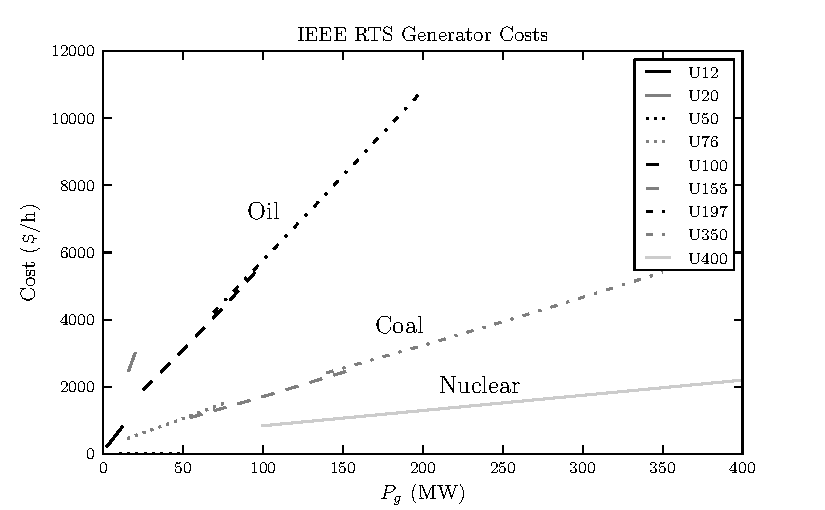
\includegraphics{figures/ieee_rts_gencosts}
	  \caption{Generator cost functions for the IEEE Reliability Test System}
	  \label{fig:ieee_rts_gencost_plot}
	\end{figure}

	\begin{figure}
	  \centering
	  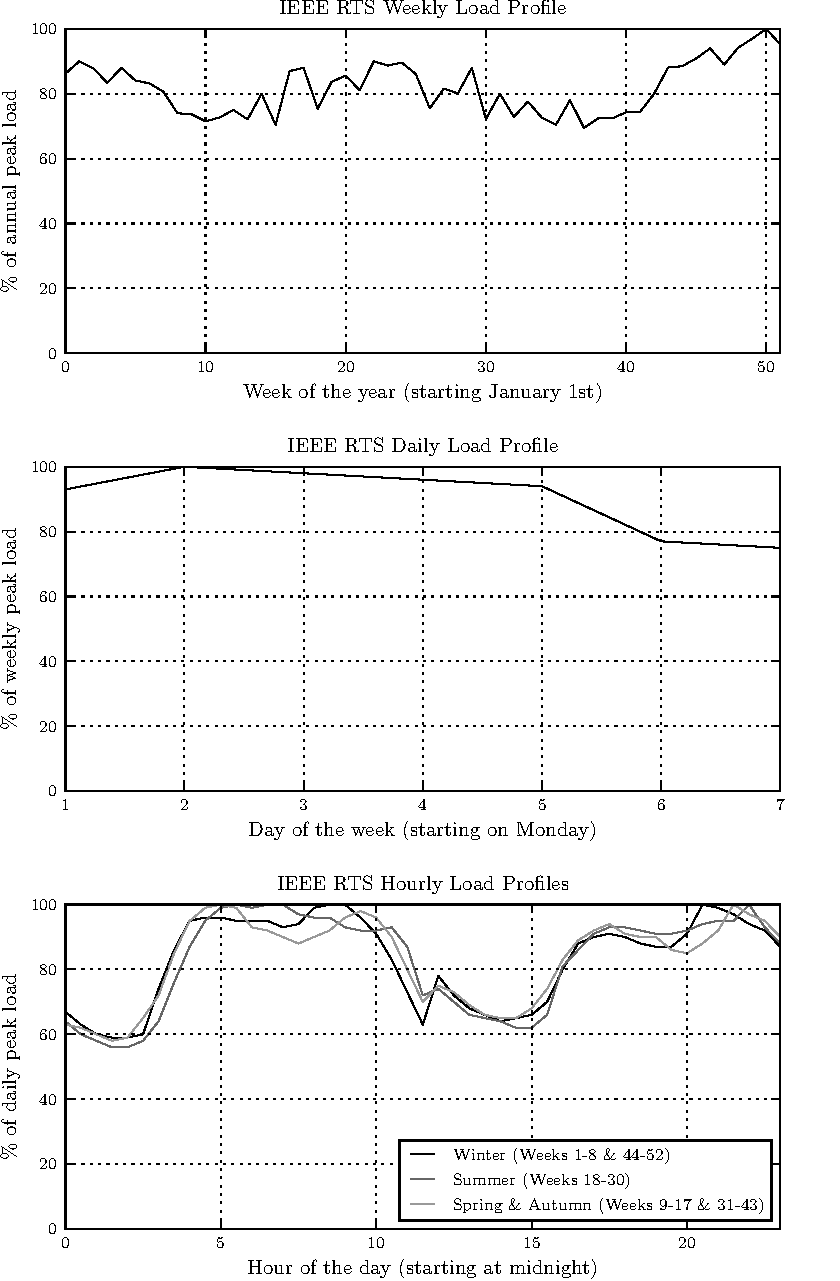
\includegraphics{figures/ieee_rts_profiles}
	  \caption{Hourly, daily and weekly load profile plots from the IEEE
	  Reliability Test System}
	  \label{fig:ieee_rts_profiles}
	\end{figure}
}{}


\begin{table}
\centering
\begin{tabular}{c|c|c|c|c|c|c|c|c}
\hline
\multirow{2}{*}{Agent} &U50 &U76 &U100 &U155 &U197 &U350 &U400 &Total \\
 &Hydro &Coal &Oil &Coal &Oil &Coal &Nuclear &(MW) \\
\hline\hline
1 & &2$\times$ & &1$\times$ & & &1$\times$ &707 \\
2 & &2$\times$ & &1$\times$ & & &1$\times$ &707 \\
3 &6$\times$ & & & &3$\times$ & & &891 \\
4 & & &3$\times$ &2$\times$ & &1$\times$ & &960 \\
\hline
\end{tabular}
\caption{Agent portfolios.}
\label{tbl:agent_portfolios}
\end{table}

The generating stock is divided into 4 portfolios (See Table
\ref{tbl:agent_portfolios}) that are each endowed to a learning agent.
Portfolios were chosen such that each agent has: a mix of base load and peaking
plant, approximately the same total generation capacity and generators in
different areas of the network.  The generator labels in Figure
\ref{fig:ieee79rts} specify the associated agent.  The synchronous condenser is
associated with a passive agent that always offers 0 MW at 0~\$/MWh (the
unit can be dispatched to provide or absorb reactive power).

\ifthenelse{\boolean{includefigures}}{\newcommand{\generatorunit}[3]{
  \node[circle,draw,thick,minimum width=6mm,#3] (#1) at (#2) {};
  \draw[thick] ($(#2)-(2mm,0)$) sin ++(1mm,1mm) cos ++(1mm,-1mm)
  sin ++(1mm,-1mm) cos ++(1mm,1mm);
}

\begin{figure}
\centering
\small
\begin{tikzpicture}[thick,label distance=0mm]
  \tikzstyle{busbar} = [rectangle,draw,fill=black!50,inner sep=0pt];
  \tikzstyle{hbus} = [busbar,minimum width=10mm,minimum height=2pt];
  \tikzstyle{vbus} = [busbar,minimum width=2pt,minimum height=10mm];
  \tikzstyle{overhead} = [-,thick];
  \tikzstyle{cable} = [thick];
  \tikzstyle{trxcircle} = [circle,draw=black,inner sep=0pt,minimum width=5mm];
  \tikzstyle{every pin edge}=[-,shorten <=1pt,thin];

\node[hbus,minimum width=15mm,label=left:Bus 1] (bus1) at (5,0) {};
\node[hbus,minimum width=15mm,label=right:Bus 2] (bus2) at (7,0) {};
\node[hbus,label=right:Bus 3] (bus3) at (0,6) {};
\node[vbus,label=above:Bus 4] (bus4) at (3,4) {};
\node[vbus,label=above:Bus 5] (bus5) at (6.5,3) {};
\node[vbus,label=above:Bus 6] (bus6) at (12,5.3) {};
\node[hbus,label=right:Bus 7] (bus7) at (11,0.5) {};
\node[vbus,label=above:Bus 8] (bus8) at (12,3) {};
\node[hbus,minimum width=20mm,label=left:Bus 9] (bus9) at (5,6) {};
\node[hbus,minimum width=20mm,label=right:Bus 10] (bus10) at (8,6) {};
\node[hbus,minimum width=20mm,label=left:Bus 11] (bus11) at (5,8) {};
\node[hbus,minimum width=20mm,label=right:Bus 12] (bus12) at (8,8) {};
\node[vbus,label={[xshift=-4mm]below:Bus 13}] (bus13) at (12,10) {};
\node[vbus,label=above:Bus 14] (bus14) at (3.5,11.5) {};
\node[hbus,minimum width=20mm,label=right:Bus 15] (bus15) at (0.5,12) {};
\node[hbus,minimum width=15mm,label=right:Bus 16] (bus16) at (0,14) {};
\node[vbus,minimum height=20mm,label=above:Bus 17] (bus17) at (-1,16) {};
\node[hbus,minimum width=20mm,label=right:Bus 18] (bus18) at (2,18) {};
\node[hbus,label=below right:Bus 19] (bus19) at (4.5,14) {};
\node[hbus,minimum width=15mm,label=below right:Bus 20] (bus20) at (7,14) {};
\node[hbus,minimum width=25mm,label=right:Bus 21] (bus21) at (5,17) {};
\node[hbus,label=right:Bus 22] (bus22) at (9,17) {};
\node[vbus,minimum height=15mm,label=above:Bus 23] (bus23) at (11,14.55) {};
\node[hbus,label=right:Bus 24] (bus24) at (0,8) {};

% Branch 1-2.
\draw[cable] ([xshift=5mm] bus1.north) -- ++(0,5mm) node[xshift=5mm,above]
{cable} -| ([xshift=-5mm] bus2.north);
% Branch 1-3.
\draw[overhead] ([xshift=-5mm] bus1.north) -- ([xshift=-5mm,yshift=5mm]
bus1.north) -- ([xshift=0mm,yshift=-5mm] bus3.south) -- (bus3.south);
% Branch 1-5.
\draw[overhead] (bus1.north) |- (bus5.west);
% Branch 2-4.
\draw[overhead] (bus2.north) -- ([yshift=5mm] bus2.north) -- ([xshift=5mm]
bus4.east) -- (bus4.east);
% Branch 2-6.
\draw[overhead] ([xshift=5mm] bus2.north) -- ([xshift=5mm,yshift=5mm]
bus2.north) -- ([xshift=-5mm,yshift=-3mm] bus6.west) -- ([yshift=-3mm]
bus6.west);
% Branche 3-9.
\draw[overhead] ([xshift=3mm] bus3.south) -- ++(0,-5mm) -| ([xshift=-5mm]
bus9.south);
% Branch 3-24.
\draw node[trxcircle,yshift=-1mm,above of=bus3] (t3-24p) {};
\draw node[trxcircle,yshift=1mm,above of=bus3] (t3-24s) {};
\draw[overhead] (bus3.north) -- (t3-24p.south);
\draw[overhead] (t3-24s.north) -- (bus24.south);
% Branch 4-9.
\draw[overhead] ([yshift=3mm] bus4.east) -- ([xshift=5mm,yshift=3mm] bus4.east)
-- ([yshift=-5mm] bus9.south) -- (bus9.south);
% Branch 5-10.
\draw[overhead] (bus5.east) -| (bus10.south);
% Branch 6-10.
\draw[overhead] (bus6.west) -| node[above right] {cable} ([xshift=5mm]
bus10.south);
% Branch 7-8.
\draw[overhead] ([xshift=-3mm] bus7.north) |- ([yshift=-3mm] bus8.west);
% Branch 8-9.
\draw[overhead] (bus8.west) -- ([xshift=-5mm] bus8.west) --
([xshift=5mm,yshift=-5mm] bus9.south) -- ([xshift=5mm] bus9.south);
% Branch 8-10;
\draw[overhead] ([yshift=3mm] bus8.west) -- ([xshift=-5mm,yshift=3mm]
bus8.west) -- ([xshift=-5mm,yshift=-10mm] bus10.south) -- ([xshift=-5mm]
bus10.south);
% Branch 9-11.
\draw node[trxcircle,yshift=-1mm,xshift=-5mm,above of=bus9] (t9-11p) {};
\draw node[trxcircle,yshift=1mm,xshift=-5mm,above of=bus9] (t9-11s) {};
\draw[overhead] ([xshift=-5mm] bus9.north) -- (t9-11p.south);
\draw[overhead] (t9-11s.north) -- ([xshift=-5mm] bus11.south);
% Branch 9-12.
\draw node[trxcircle,yshift=-1mm,xshift=-5mm,node distance=7mm,below of=bus12]
(t9-12p) {};
\draw node[trxcircle,yshift=1mm,xshift=-5mm,node distance=7mm,below of=bus12]
(t9-12s) {};
\draw[overhead] ([xshift=5mm] bus9.north) -- ([xshift=5mm,yshift=3mm]
bus9.north) -- ([yshift=-3mm] t9-12p.south) -- (t9-12p.south);
\draw[overhead] (t9-12s.north) -- ([xshift=-5mm] bus12.south);
% Branch 10-11.
\draw node[trxcircle,yshift=-1mm,xshift=5mm,node distance=7mm,below of=bus11]
(t10-11p) {};
\draw node[trxcircle,yshift=1mm,xshift=5mm,node distance=7mm,below of=bus11]
(t10-11s) {};
\draw[overhead] ([xshift=-5mm] bus10.north) -- ([xshift=-5mm,yshift=3mm]
bus10.north) -- ([yshift=-3mm] t10-11p.south) -- (t10-11p.south);
\draw[overhead] (t10-11s.north) -- ([xshift=5mm] bus11.south);
% Branch 10-12.
\draw node[trxcircle,yshift=-1mm,xshift=5mm,above of=bus10] (t10-12p) {};
\draw node[trxcircle,yshift=1mm,xshift=5mm,above of=bus10] (t10-12s) {};
\draw[overhead] ([xshift=5mm] bus10.north) -- (t10-12p.south);
\draw[overhead] (t10-12s.north) -- ([xshift=5mm] bus12.south);
% Branch 11-13.
\draw[overhead] ([xshift=5mm] bus11.north) -- ([xshift=5mm,yshift=5mm]
bus11.north) -- ([xshift=-5mm] bus13.west) -- (bus13.west);
% Branch 11-14.
\draw[overhead] ([xshift=-5mm] bus11.north) |- ([yshift=-3mm] bus14.east);
% Branch 12-13.
\draw[overhead] ([xshift=-5mm] bus12.north) -- ([xshift=-5mm,yshift=7mm]
bus12.north) -- ([xshift=-5mm,yshift=-3mm] bus13.west) -- ([yshift=-3mm]
bus13.west);
% Branch 12-23.
\draw[overhead] ([xshift=5mm] bus12.north) |- ([yshift=-5mm] bus23.west);
% Branch 13-23.
\draw[overhead] ([yshift=3mm] bus13.west) -- ([xshift=-5mm,yshift=3mm]
bus13.west) |- ([yshift=-5mm] bus23.east);
% Branch 14-16.
\draw[overhead] ([yshift=3mm] bus14.west) -- ([xshift=-6mm,yshift=3mm]
bus14.west) |- ([xshift=5mm,yshift=-5mm] bus16.south) -- ([xshift=5mm]
bus16.south);
% Branch 15-16.
\draw[overhead] ([xshift=-5mm] bus15.north) -- (bus16.south);
% Branches 15-21.
\draw[overhead] (bus15.north) -- ([yshift=5mm] bus15.north) -- ([yshift=-10mm]
bus21.south) -- (bus21.south);
\draw[overhead] ([xshift=5mm] bus15.north) -- ([xshift=5mm,yshift=5mm]
bus15.north) -- ([xshift=5mm,yshift=-10mm] bus21.south) -- ([xshift=5mm]
bus21.south);
% Branch 15-24.
\draw[overhead] ([xshift=-5mm] bus15.south) -- (bus24.north);
% Branch 16-17.
\draw[overhead] ([xshift=-5mm] bus16.north) |- ([yshift=-5mm] bus17.east);
% Branch16-19.
\draw[overhead] ([xshift=5mm] bus16.north) -- ([xshift=5mm,yshift=5mm]
bus16.north) -| ([xshift=-3mm] bus19.north);
% Branch 17-18.
\draw[overhead] ([yshift=5mm] bus17.east) -| ([xshift=-5mm] bus18.south);
% Branch 17-22.
\draw[overhead] (bus17.east) -- ([xshift=20mm] bus17.east) -- ([xshift=20mm,
yshift=-5mm] bus17.east) -| ([xshift=3mm] bus22.south);
% Branches 18-21.
\draw[overhead] (bus18.south) -- ([yshift=-20mm] bus18.south) -|
([xshift=-5mm] bus21.south);
\draw[overhead] ([xshift=5mm] bus18.south) -- ([xshift=5mm,yshift=-15mm]
bus18.south) -| ([xshift=-10mm] bus21.south);
% Branches 19-20.
\draw[overhead] (bus19.north) -- ([yshift=10mm] bus19.north) -|
([xshift=-1.5mm] bus20.north);
\draw[overhead] ([xshift=3mm] bus19.north) -- ([xshift=3mm,yshift=5mm]
bus19.north) -| ([xshift=-4.5mm] bus20.north);
% Branches 20-23.
\draw[overhead] ([xshift=1.5mm] bus20.north) |- ([yshift=5mm] bus23.west);
\draw[overhead] ([xshift=4.5mm] bus20.north) |- (bus23.west);
% Branch 21-22.
\draw[overhead] ([xshift=10mm] bus21.south) -- ([xshift=10mm,yshift=-7.5mm]
bus21.south) -| ([xshift=-3mm] bus22.south);

% Generator @ Bus 1.
\generatorunit{gen1}{4.5,-0.8}{label=left:192 MW,pin={[pin distance=12mm,text
centered,text width=10.5mm]165:2$\times$U20 2$\times$U76}};
\draw[overhead] ([xshift=-5mm] bus1.south) -- (gen1.north);
% Generator @ Bus 2.
\generatorunit{gen2}{7.5,-0.8}{label=right:192 MW,pin={[pin distance=12mm,text
centered,text width=10.5mm]15:2$\times$U20 2$\times$U76}};
\draw[overhead] ([xshift=5mm] bus2.south) -- (gen2.north);
% Generator @ Bus 7.
\generatorunit{gen3}{11,-0.3}{label=right:300 MW,pin=below:3$\times$U100};
\draw[overhead] (bus7.south) -- (gen3.north);
% Generator @ Bus 13.
\generatorunit{gen4}{12.3,10.9}{label=above:591 MW,pin={[pin distance=8mm]
left:3$\times$U197}};
\draw[overhead] ([yshift=3mm] bus13.east) -- ([yshift=3mm,xshift=2.5mm]
bus13.east) -- (gen4.south);
% Generator @ Bus 14.
\generatorunit{gen5}{4.3,11.8}{label={[text justified,text
width=15mm]right:Synch. Cond.}}; \draw[overhead] ([yshift=3mm] bus14.east) --
(gen5.west);
% Generator @ Bus 15.
\generatorunit{gen6}{0.5,11.2}{label={[text centered,text width=10mm]below:215 MW},
pin={[pin distance=5mm,text centered,text width=15mm]-70:5$\times$U12
1$\times$U155}}; \draw[overhead] (bus15.south) -- (gen6.north);
% Generator @ Bus 16.
\generatorunit{gen7}{0.0,15}{label=right:155 MW};
\draw[overhead] (bus16.north) -- (gen7.south);
% Generator @ Bus 18.
\generatorunit{gen8}{1.5,18.8}{label=left:400 MW,pin={[pin distance=6mm]below
left:Nuclear}}; \draw[overhead] ([xshift=-5mm] bus18.north) -- (gen8.south);
% Generator @ Bus 21.
\generatorunit{gen9}{5,17.8}{label=right:400 MW,pin={above right:Nuclear}};
\draw[overhead] (bus21.north) -- (gen9.south);
% Generator @ Bus 22.
\generatorunit{gen10}{9,17.8}{label=right:300 MW,pin={above:Hydro, 6$\times$U50}};
\draw[overhead] (bus22.north) -- (gen10.south);
% Generator @ Bus 23.
\generatorunit{gen11}{11.8,15.05}{label=below:660 MW,pin={[text centered,text
width=15mm]above:2$\times$U155 1$\times$U350}};
\draw[overhead] ([yshift=5.05mm] bus23.east) -- (gen11.west);

% Load @ Bus 1.
\draw[loadline] ([xshift=5mm] bus1.south) -- ++(0,-0.8) node[text centered,text
width=10mm,below] {108 MW};
% Load @ Bus 2.
\draw[loadline] ([xshift=-5mm] bus2.south) -- ++(0,-0.8) node[text
centered,text width=10mm,below] {97 MW};
% Load @ Bus 3.
\draw[loadline] ([xshift=-3mm] bus3.south) -- ++(0,-0.8) node[text
centered,text width=10mm,below] {108 MW};
% Load @ Bus 4.
\draw[loadline] ([yshift=-3mm] bus4.east) -- ++(3mm,0) -- ++(0,-0.8)
node[below] {74 MW};
% Load @ Bus 5.
\draw[loadline] ([yshift=-3mm] bus5.east) -- ++(3mm,0) --
++(0,-0.8) node[below] {71 MW};
% Load @ Bus 6.
\draw[loadline] (bus6.east) -- ++(3mm,0) -- ++(0,-0.8) node[below] {136 MW};
% Load @ Bus 7.
\draw[loadline] ([xshift=3mm] bus7.north) -- ++(0,0.8) node[right] {125 MW};
% Load @ Bus 8.
\draw[loadline] (bus8.east) -- ++(3mm,0) -- ++(0,-0.8) node[left] {171 MW};
% Load @ Bus 9.
\draw[loadline] ([xshift=2.5mm] bus9.south) -- ++(0,-1) node[below] {175 MW};
% Load @ Bus 10.
\draw[loadline] ([xshift=7.5mm] bus10.north) -- ++(0,3mm) -- ++(8mm,0)
node[above right] {195 MW};
% Load @ Bus 13.
\draw[loadline] ([yshift=-3mm] bus13.east) -- ++(2.5mm,0) -- ++(0,-1)
node[below] {265 MW};
% Load @ Bus 14.
\draw[loadline] ([yshift=-3mm] bus14.west) -- ++(-3mm,0) -- ++(0,-0.8)
node[below] {194 MW};
% Load @ Bus 15.
\draw[loadline] ([xshift=7mm] bus15.south) -- ++(0,-0.8) node[right]
{317 MW};
% Load @ Bus 16.
\draw[loadline] ([xshift=-5mm] bus16.south) -- ++(0,-0.8) node[text centered,
text width=10mm,below] {100 MW};
% Load @ Bus 18.
\draw[loadline] ([xshift=5mm] bus18.north) -- ++(0,0.8) node[right] {333 MW};
% Load @ Bus 19.
\draw[loadline] (bus19.south) -- ++(0,-0.8) node[right] {181 MW};
% Load @ Bus 20.
\draw[loadline] (bus20.south) -- ++(0,-0.8) node[below] {128 MW};

% Area voltage labels.
\node[draw] at (1,2) {\normalsize{138 kV}};
\node[draw] at (6.5,10.3) {\normalsize{230 kV}};

\end{tikzpicture}
\caption{IEEE Reliability Test System}
\label{fig:ieee79rts}
\end{figure}}{}

Markups on marginal cost are restricted a maximum of 30\% and discrete markups
of 0, 15\% or 30\% are defined for value function based methods.  Upto 20\% of
the total capacity of each generator can be withheld and discrete withholds of
0~or~20\% are defined.  Initially only one offer per generator is required, but
this is increased to two in order to explore the effect of increased offer
flexibility.
% Agent~3 has the largest discrete action space with XX
% possible actions to be explored in each state.

The environment state for all algorithm tests consists of a forecast of the
total system demand for the next period.  The system demand follows an hourly
profile that is adjusted according to the day of the week and the time of year.
The profiles are taken from the RTS and are illustrated in Figure
\ref{fig:ieee_rts_profiles}.  For tests of value function based methods and the
Roth-Erev learning algorithm, the continuous state is divided into 3 discrete
states of equal size, that allow differentiation between low, medium and peak
demand.

To investigate the exploration of constraints, AC optimal power flow is used and
the state vector for agents using policy gradient methods is optionally adjusted
to combine the demand forecast with voltage constraint Lagrangian multipliers
for all generator buses and the voltage magnitude at all other buses.  Lagrangian
multipliers are used as generators typically fix the voltage at their associated
bus.  Branch flows are not included in the state vector as the flow limits in
the RTS are high and are typically not reached at peak demand.  Generator
capacity limits are binding in most states of the RTS, but the output of other generators is
deemed to be hidden from agents.

The nodal marginal pricing scheme is used and cleared offer prices are
determined by the Lagrangian multiplier on the power balance constraint for the
bus at which the generator associated with the offer is connected.

Typical parameter values are used for each of the algorithms.  Learning rates
are set low and exploration parameters decay slowly due to the length
and complexity of each simulation.  For Q-learning $\alpha=0.2$, $\gamma=0.99$
and $\epsilon$-greedy action selection is used with $\epsilon=0.9$ and
$d=0.999$. For Roth-Erev learning $\epsilon=0.55$, $\phi=0.3$ and Boltzmann
action selection is used with $\tau=100$ and $d=0.999$.

Two-layer neural networks with linear input and output nodes, no bias nodes and
randomised initial connection weights are used for policy function
approximation.  The initial exploration rate $\sigma=0$ for both policy
gradient methods and decays according to Equation (\ref{eq:sigmadecay}) with
$d=0.995$ and $\sigma_n=-0.5$.  Constant learning rates are used in each
simulation with $\gamma=0.01$ for REINFORCE and $\gamma=0.005$ for ENAC.

\section{Simulation Results}
Each agent's rewards are recorded for a simulated year of 364 trading episodes,
each consisting of 24 interactions.  To compare algorithms, the average reward
for each hour of the day is calculated for each agent and plotted.  Only results
for agents 1 and 4 are given as agents 1 and 2 have identical portfolios and
most of agent 3's portfolio consists of Hydro plant with zero cost.  The method
of applying percentage markups on marginal cost does not work for generators
with zero cost and almost identical results are found for all algorithms.

\ifthenelse{\boolean{includefigures}}{
  \begin{figure}
    \centering
    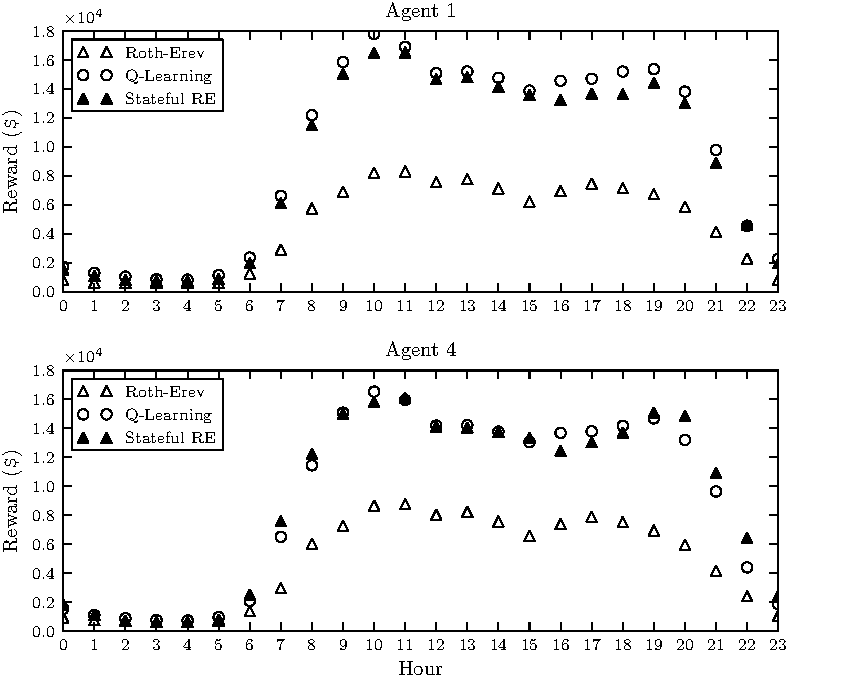
\includegraphics{figures/fig6_1}
    \caption{Modified Roth-Erev compared with Stateful Roth-Erev.}
    \label{fig:6_1}
  \end{figure}
}

Figure \ref{fig:6_1} compares the modified Roth-Erev method with the Stateful
Roth-Erev method.  The plots show average rewards for agents 1 and 4 when
using Q-learning and the two Roth-Erev variants.

\ifthenelse{\boolean{includefigures}}{
  \begin{figure}
    \centering
    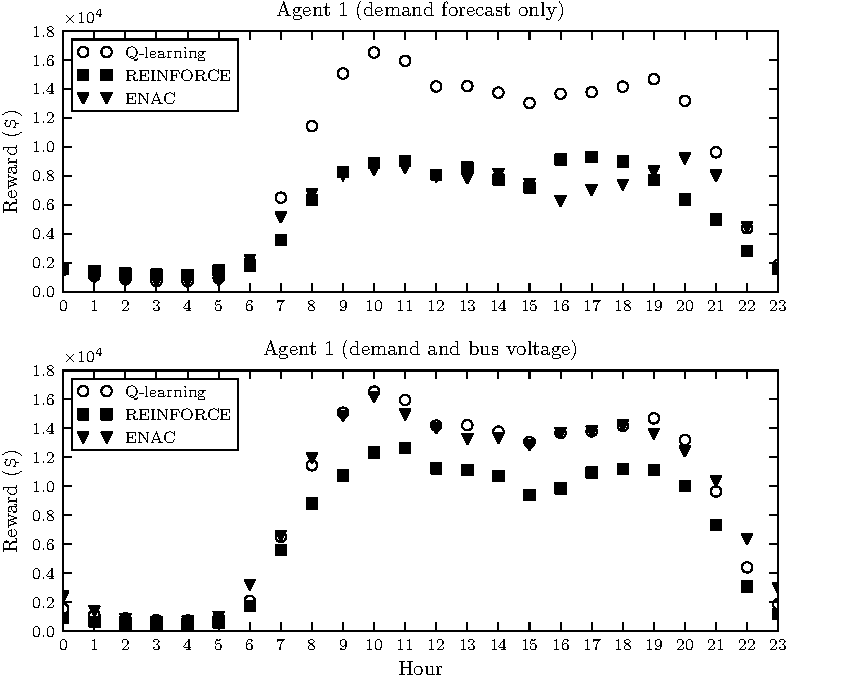
\includegraphics{figures/fig6_2_a1}
    \caption{Average rewards for agent 1 under two state configurations.}
    \label{fig:6_2_a1}
  \end{figure}

  \begin{figure}
    \centering
    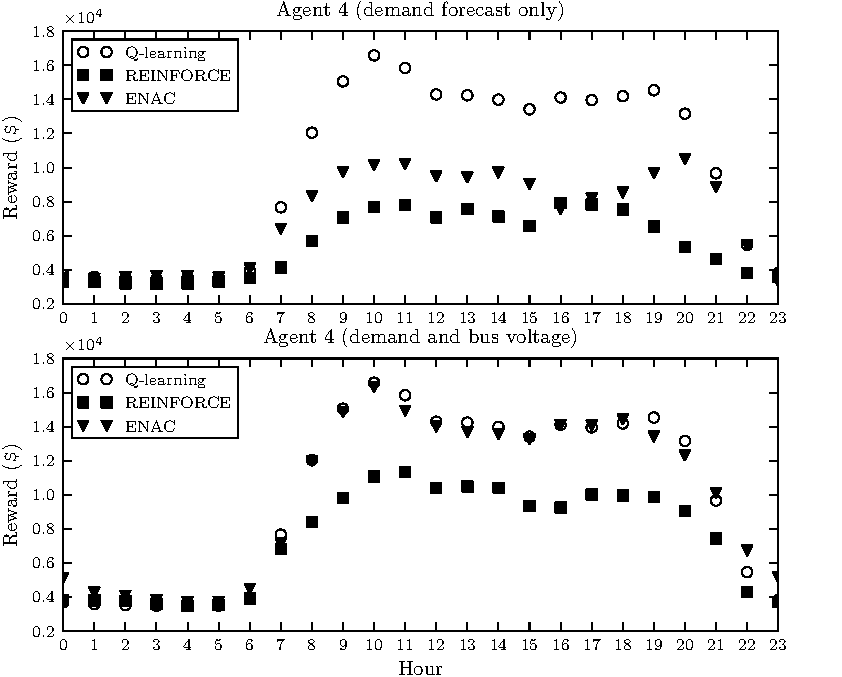
\includegraphics{figures/fig6_2_a4}
    \caption{Average rewards for agent 4 under two state configurations.}
    \label{fig:6_2_a4}
  \end{figure}
}

Figure \ref{fig:6_2_a1} and Figure \ref{fig:6_2_a4} compare policy gradient
methods under two state vector configurations.  Figure \ref{fig:6_2_a1} concerns
agent 1 and show the average reward received for a state vector consisting
solely of a demand forecast and for a combined demand forecast and bus voltage
profile state vector.  Figure \ref{fig:6_2_a4} shows average rewards for
agent~4 under the same configurations.

\ifthenelse{\boolean{includefigures}}{
  \begin{figure}
    \centering
    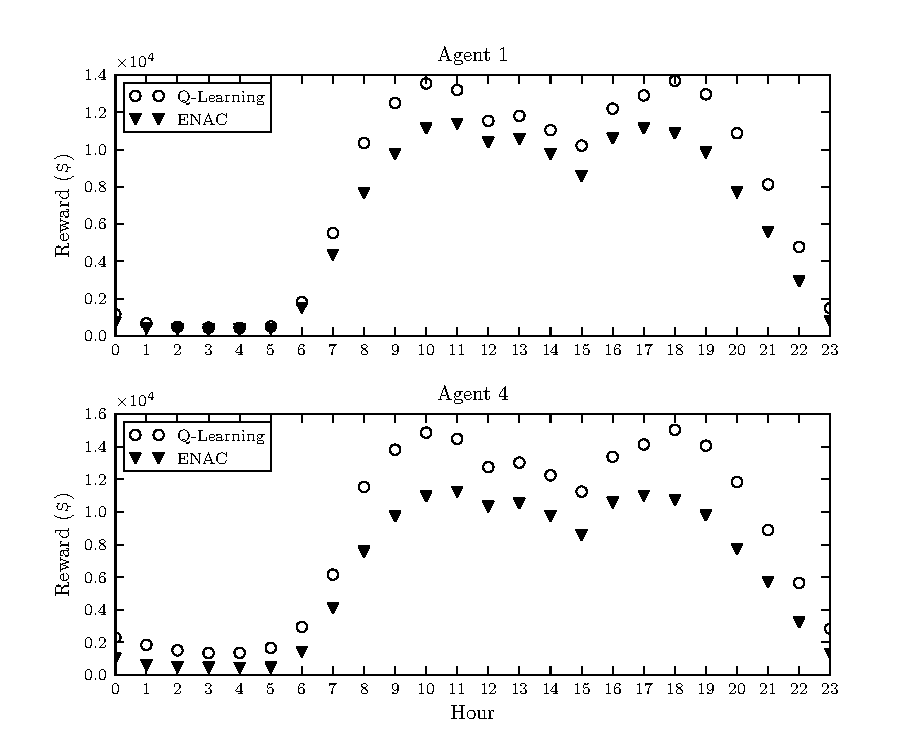
\includegraphics{figures/fig6_3}
    \caption{Average rewards for two offers per generator.}
    \label{fig:6_3}
  \end{figure}
}

Figure \ref{fig:6_3} shows average rewards for agents 1 and 4 from a repeat of
the bus voltage profile state simulation, but with two offers required per
generator.  Due to time constraints and limited simulation resources only
results for Q-learning and ENAC are given.

\section{Discussion and Critical Analysis}
\label{sec:discuss}
Agents with a discrete environment have 216 possible actions to choose from in
each state when required to submit one offer per generator.  Figure
\ref{fig:6_1} shows that, using Q-learning, the agents are able to learn an
effective policy that yields increased profits using two different portfolios.
The importance of utilising environment state data in a dynamic electricity
setting is illustrated by the differences in average reward received by the
modified Roth-Erev method and the Stateful Roth-Erev method.  The optimal action
for an agent depends upon the current system load and the stateless Roth-Erev
formulation is unable to interpret this.  Stateful Roth-Erev can be seen to
achieve approximately the same performance as Q-learning.

Including bus voltage constraint data in the state for a discrete environment
would result in a state space of impractical size, but including it in a
continuous environment was straight-forward.  The results show that ENAC
achieves greater profits when presented with a combined demand forecast and bus
voltage state vector.  REINFORCE performs less well than ENAC, but also shows
improvement over the pure forecast case.  ENAC achieves equivalent, but not
greater performance than Q-learning in all periods of the trading day when
using the voltage data.  It is not able to use the additional state information
to any further advantage, but does learn a profitable policy.
% In robotics, policy gradient methods are typically used with neural networks
% with more that one input node and the effect of this network structure deserves
% further investigation.

Simply changing the number of offers required to be submitted for each generator
from 1 to 2, increases the number of discrete action possibilities in each state
to 46,656.  Figure \ref{fig:6_3} shows that Q-learning is still able to achieve
a similar level of reward that achieved under the one offer case.  The
profitability for both methods is degraded, but ENAC receives significantly
lower average reward when required to produce a larger action vector and is not
able to use the increased flexibility in its offer structure to any advantage.

\section{Summary}
No evidence has been found to suggest that policy gradient methods can be used
to exploit complex constraints in a power system model.  However, they have been
shown to operate better with large state vectors.  Some limitations of the
standard Roth-Erev formulation in an dynamic environment have been
demonstrated. Q-learning was able to produce an effective policy in all simulations, including one
involving a relatively large action space that saw severely degraded
performance from a policy gradient method.

AC optimal power flow adds enormously to simulation times when analysing an
entire year of hourly trading interactions.  The addition of bus voltage data
to the state vector improved the performance of the policy gradient methods, but it has
not been show if the same could not be achieved by perhaps using bus voltage
angles from a DC optimal power flow.
